\documentclass[french]{beamer}
\usepackage[T1]{fontenc}
\usepackage[utf8]{inputenc}
\usepackage{amstext}
\usepackage{graphicx}
\usepackage[font=small,labelfont=bf]{caption}


\usetheme{CambridgeUS}

\title{Projet TouDou}
<<<<<<< HEAD
\author{Équipe MOE Crossfit : \\Barbier Thomas, Gama Abel, Robcis Quentin, Pawlak Thibault
=======
\author{Équipe MOE Crossfit : \\Barbier Thomas, Gama Abel, Robcis Quentin, Pawlak Thibault \\
>>>>>>> 98ea522da6858c3fa1de0477aa833dc385800d23
\vspace{0.5}
Équipe MOA OneAppToRuleThemAll: \\De Fillipis Michael, Lerogeron Hugo, Ridel Morgan }
\institute[]{INSA de Rouen}
\date{\today}

\begin{document}

\section{Présentation}
\begin{frame}
\titlepage
\end{frame}

\section{Sommaire}
\begin{frame}
\tableofcontents
\end{frame}

\section{Cahier des charges}
\begin{frame}
\begin{itemize}
  \item Agenda
  \item Liste des tâches
  \item Partage des tâches
  \item Priorisation des tâches
  \item Exportation
\end{itemize}
\end{frame}

\section{Démarche suivie}
\begin{frame}
  \begin{center}
  \begin{minipage}[c]{0.6\linewidth}%
   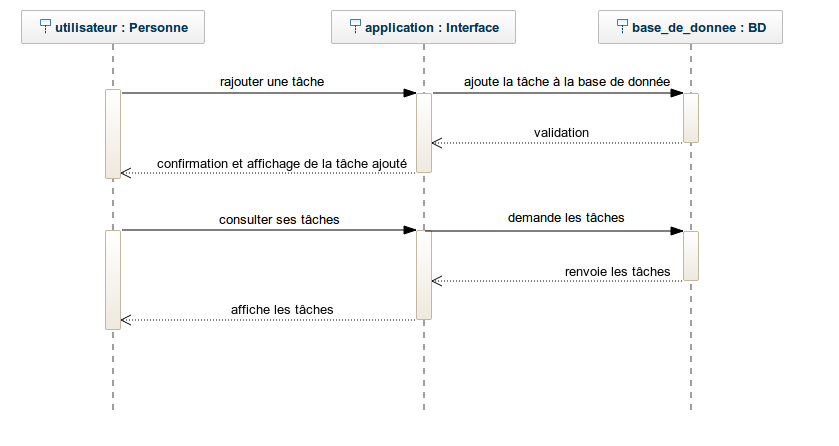
\includegraphics[width=1\linewidth]{dss} \captionof{figure}{Diagramme de séquence pour la liste des tâches} %
  \end{minipage}
\end{center}
\end{frame}

\begin{frame}
  \begin{center}
  \begin{minipage}[c]{0.6\linewidth}%
   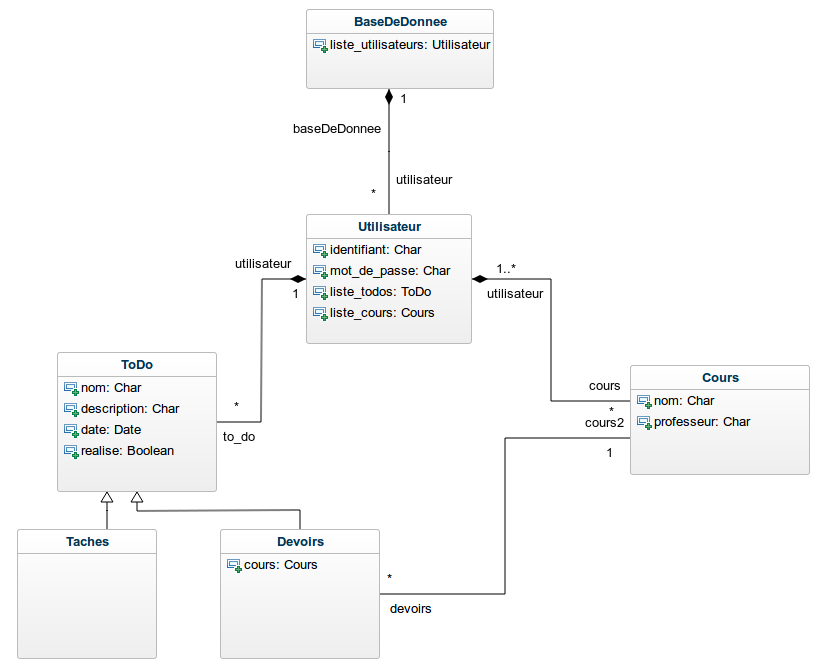
\includegraphics[width=1\linewidth]{dcp} \captionof{figure}{Diagramme de classe participante du projet} %
  \end{minipage}
\end{center}
\end{frame}

\begin{frame}
  \begin{center}
  \begin{minipage}[c]{0.6\linewidth}%
   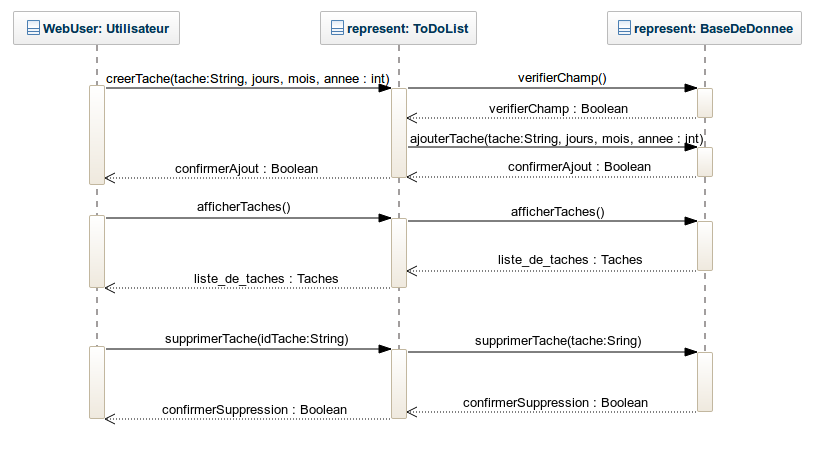
\includegraphics[width=1\linewidth]{dsa} \captionof{figure}{Diagramme de séquence d'analyse} %
  \end{minipage}
\end{center}
\end{frame}

\begin{frame}
  \begin{center}
  \begin{minipage}[c]{0.6\linewidth}%
   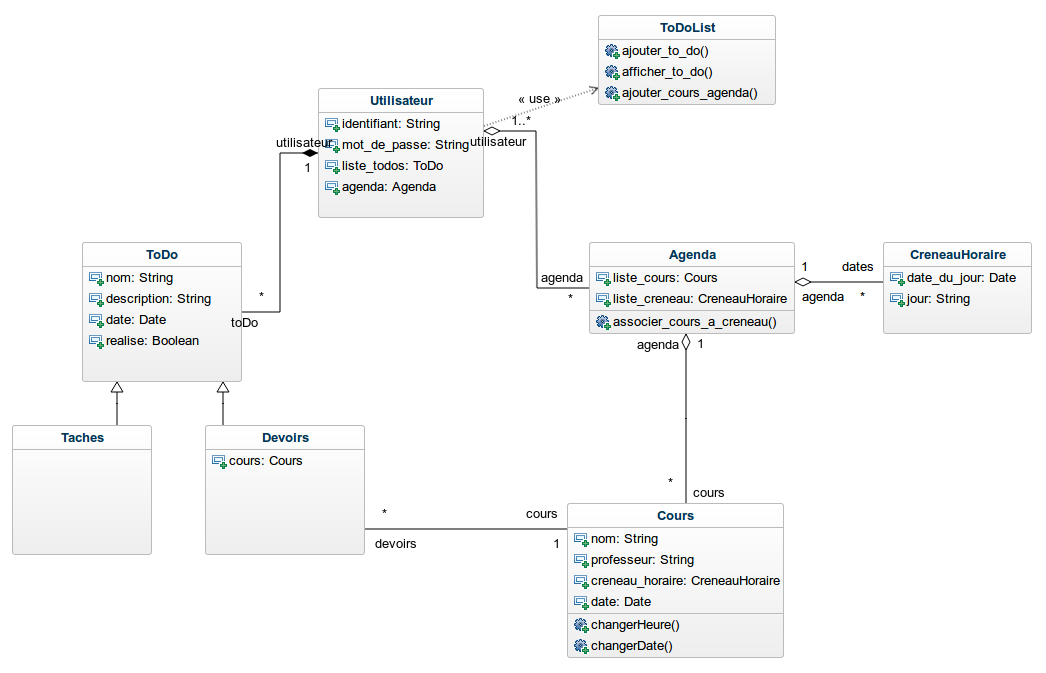
\includegraphics[width=1\linewidth]{mdd} \captionof{figure}{Modèle du domaine} %
  \end{minipage}
\end{center}
\end{frame}

\section{Prototype}
\begin{frame}
  \begin{center}
  \begin{minipage}[c]{0.4\linewidth}%
   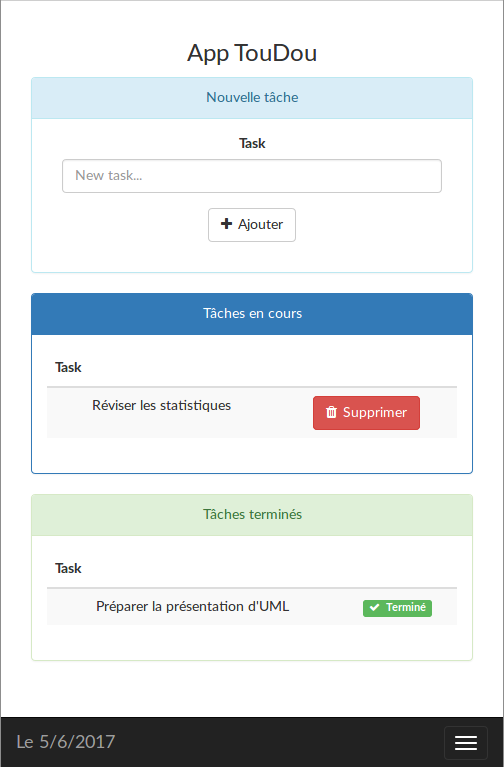
\includegraphics[width=1\linewidth]{prototype} \captionof{figure}{Une capture d'écran du prototype de liste des tâches} %
  \end{minipage}
\end{center}
\end{frame}

\section{Conclusion}
\begin{frame}
\begin{center}
  Prototype visible sur : \url{https://umlp.github.io/filr2017pmoe-crossfit/prototype.html}\\
  \vspace{0.5cm}
  Si c'était à refaire\dots
\end{center}
\end{frame}
\end{document}
